\documentclass[pdflatex,sn-mathphys-num]{sn-jnl}% Math and Physical Sciences Numbered


\usepackage{graphicx}%
\usepackage{multirow}%
\usepackage{amsmath,amssymb,amsfonts}%
\usepackage{amsthm}%
\usepackage{mathrsfs}%
\usepackage[title]{appendix}%
\usepackage{xcolor}%
\usepackage{textcomp}%
\usepackage{manyfoot}%
\usepackage{booktabs}%
\usepackage{algorithm}
\usepackage{algorithmicx}
\usepackage{algpseudocode}
\usepackage{multicol}
\usepackage{fancyvrb}
\usepackage{geometry}
\usepackage{titlesec}
\usepackage{xcolor}
\usepackage{parskip}
\usepackage[backend=biber,style=apa]{biblatex} % or use another style
\addbibresource{references.bib} % your .bib file
\usepackage{hyperref}
\usepackage{fontawesome5} % For the GitHub icon
\usepackage[justification=centering]{caption}
\usepackage[linesnumbered,ruled,vlined]{algorithm2e}
\setlength{\topmargin}{-0.4in}
\setlength{\textheight}{9in}
\usepackage{comment}
\usepackage{listings}%
% In your preamble:
\usepackage{enumitem} % For custom list formatting
\newlist{questions}{enumerate}{1}
\setlist[questions,1]{
  label=\textbf{Q\arabic*:}, % Label format "Q1:", "Q2:", ...
  leftmargin=2em,           % Indent spacing
  itemsep=1em               % Space between questions
}



%%%%


%% as per the requirement new theorem styles can be included as shown below
\theoremstyle{thmstyleone}%
\newtheorem{theorem}{Theorem}%  meant for continuous numbers
%%\newtheorem{theorem}{Theorem}[section]% meant for sectionwise numbers
%% optional argument [theorem] produces theorem numbering sequence instead of independent numbers for Proposition
\newtheorem{proposition}[theorem]{Proposition}%
%%\newtheorem{proposition}{Proposition}% to get separate numbers for theorem and proposition etc.

\theoremstyle{thmstyletwo}%
\newtheorem{example}{Example}%
\newtheorem{remark}{Remark}%

\theoremstyle{thmstylethree}%
\newtheorem{definition}{Definition}%

\raggedbottom

\usepackage{amssymb}

% Code Packages

\usepackage{listings}
\usepackage{xcolor}

\definecolor{headerbackground}{rgb}{1, 1, 1}
\definecolor{rulecolor}{rgb}{0.7, 0.7, 0.7}

% Define C keywords including standard library functions
\lstdefinestyle{algorithmstyle}{
  backgroundcolor=\color{white},
  basicstyle=\ttfamily\scriptsize,
  keywordstyle=\bfseries, % Bold for keywords
  commentstyle=\itshape, % Italic for comments
  stringstyle=,
  numberstyle=\tiny,
  numbers=left,
  numbersep=10pt,
  breaklines=true,
  frame=trbl,
  framerule=0.8pt,
  rulecolor=\color{rulecolor},
  framesep=5pt,
  xleftmargin=15pt,
  xrightmargin=5pt,
  language=C, % This is crucial
  tabsize=2,
  showstringspaces=false,
  alsoletter={\_},
  morekeywords={printf, scanf, malloc, free, sizeof, puts, gets}, % Add standard library functions
}

\newcommand{\codeheader}[1]{%
  \noindent%
  \fcolorbox{rulecolor}{headerbackground}{%
    \makebox[\dimexpr\linewidth-2\fboxsep-2\fboxrule][l]{%
      \textbf{Code:} \ttfamily{#1}%
    }%
  }%
  \vspace{-0.5\baselineskip}
}

\newcommand{\magn}[1]{
     \left[#1\right]
}

\begin{document}

\title[Article Title]{Fuente de Voltaje Lineal con Protección Corto-Circuito }


\author{\fnm{Contreras R} \sur{Orlando},\fnm{ Garcia B} \sur{Iker},\fnm{ Lara H} \sur {Kevin}, \fnm{ Navarrete V Iker}}\email{\{al348390,al307630, al464376, al300304\}@edu.uaa.mx}



\affil[3]{\orgdiv{Department of Electronic Systems}, \orgname{UAA}, \orgaddress{\street{Av. Universidad 940}, \city{Aguascalientes}, \postcode{20131}, \state{Aguascalientes}, \country{México}}}

%%==================================%%
%% Sample for unstructured abstract %%
%%==================================%%

\abstract{This project presents the design of a linear DC power supply with 3.3V, 5V and 0–15V adjustable outputs, including short-circuit protection. A transformer, full-wave rectifier, filtering stage and LM317 regulators were implemented. Short-circuit detection is achieved using a shunt resistor and comparator, triggering a latch that disconnects the load to prevent damage. Tests confirmed stable voltage regulation and correct protection activation.}


%% me dices si ocupas ayuda con algo ire a desyunar oki probecho
%%================================%%
%% Sample for structured abstract %%
%%================================%%

\keywords{Power Supply, LM317, Linear Regulator, Comparator, Electronics.}

%%\pacs[JEL Classification]{D8, H51}

%%\pacs[MSC Classification]{35A01, 65L10, 65L12, 65L20, 65L70}

\maketitle

\section{Marco Teórico}
La mayor parte de los dispositivos electrónicos requieren de voltajes continuos para operar. Las baterías son una opción muy poco viable debido a su vida útil y la tensión de la red eléctrica tiende a ser muy grande para algunos. Esta tensión puede ser manipulada fácilmente usando un transformador y circuitos rectificadores, los que sumados a un dispositivo regulador proporcionan diferentes valores de tensión. El diagrama completo esquematizado de la fuente se puede observar en la figura \ref{fig:fag0}.
\begin{figure}[!h]
    \centering
    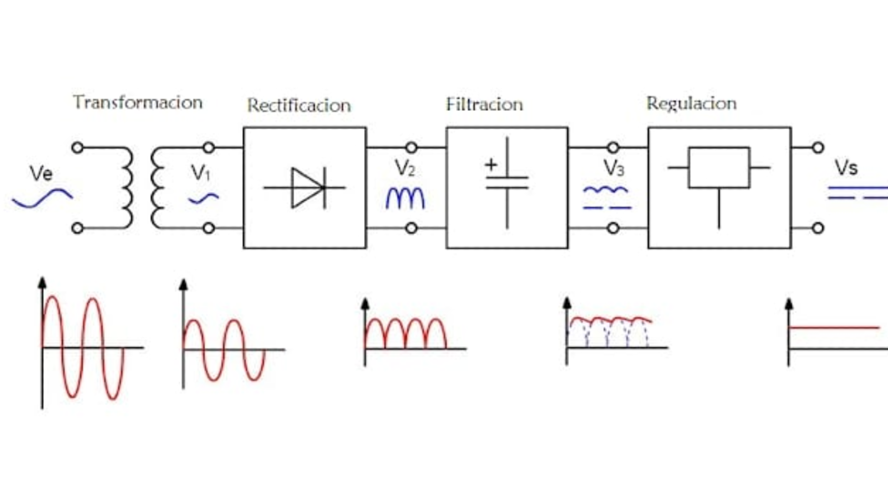
\includegraphics[width=0.38\linewidth]{src/et2.png}
    \caption{Etapas de una fuente de alimentación}
    \label{fig:fag0}
\end{figure}

\subsection{Transformador}
La estructura básica de un transformador se compone de 2 devanados; el primario y el secundario, ambos aislados y compartiendo el mismo núcleo como se muestra en la \ref{fig:fag1}, el cual permite concentrar y dirigir el flujo magnético (Pérez-Londoño, 2022). Este componente se basa en el principio de inducción electromagnética y permite la transferencia de energía de un componente a otro. Cuando se aplica corriente alterna al devanado primario, éste genera un campo magnético variable en el núcleo. \\

Ese campo magnético induce una tensión en el devanado secundario, transfiriendo energía sin conexión conductora directa entre primaria y secundaria. Gracias a la relación de vueltas entre primario y secundario, el transformador puede elevar (step-up) o reducir (step-down) la tensión (o corriente) según lo requiera la aplicación.

\begin{figure}[!h]
    \centering
        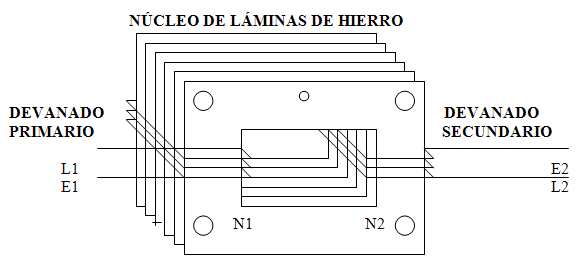
\includegraphics[width=0.75\linewidth]{src/I1.png}
    \caption{Estructura básica del transformador}
    \label{fig:fag1}
\end{figure}

\subsection{Rectificador}
El rectificador de onda completa, formado con 4 diodos o también conocido como puente de diodos, permite utilizar toda la energía disponible de los semiciclos negativos en contraparte con los rectificadores de media onda (Rendón, s.f.; Miyara, 2002). El funcionamiento es bastante simple, cuando el voltaje de entrada es positivo, los diodos D1 y D2 ilustrados en la Fig. \ref{fig:fag2} conducen debido a que se polarizan de forma directa, mientras que los diodos de D3 y D4 no conducen. 

Sin embargo, pasa lo contrario al aplicar un voltaje negativo; es decir el semiciclo negativo de la fuente de entrada, de esta manera D3 y D4 se polarizarán de forma directa y los diodos D1 y D2 no conducen. 

\begin{figure}[!h]
    \centering
    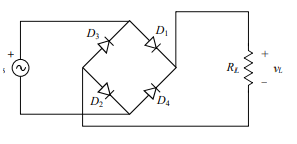
\includegraphics[width=0.7\linewidth]{src/Rectif.png}
    \caption{Rectificador de Onda Completa}
    \label{fig:fag2}
\end{figure}

El funcionamiento observado al implementarlo en una señal de entrada produce la señal de la Fig. \ref{fig:fag3}, en donde se observa un aprovechamiento total de la señal de entrada y una corriente unidireccional.

\begin{figure}[!h]
    \centering
    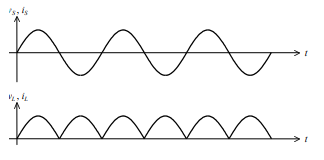
\includegraphics[width=0.5\linewidth]{src/Rectificada.png}
    \caption{Aprovechamiento de los semiciclos negativos y positivos de la señal de entrada.}
    \label{fig:fag3}
\end{figure}

\subsection{Regulador}
El rectificador distorsiona la señal de entrada y permite que su salida tenga componentes de continua (Huircán, 2012). A partir de aquí es importante agregar un filtro que rechace los armónicos de la salida del rectificador, a partir de dicho filtro la señal queda con un rizado, el cual se corrige por el regulador y logra obtener una impedancia adecuada con el propósito de lograr una tensión específica independientemente de la carga en la salida del regulador.

Existen algunos requerimientos para el uso del regulador. 	
\begin{itemize}
    \item Mantener la tensión de salida constante independiente de las fluctuaciones de la entrada y la temperatura. 
    \item Mantener la tensión constante de salida, a las exigencias de corriente de carga. 
    \item El voltaje de salida no debe contener componentes alternos (ripple =0) 
    \item La fuente debe poseer un sistema para limitar la corriente de salida (protección).
\end{itemize}

A partir del voltaje de entrada sin regular, podemos definir la razón del voltaje de salida, en base a los cambios en los coeficientes de estabilización y el coeficiente de temperatura. Se ilustra a continuación, la relación entre el voltaje de entrada y el considerado para el rizo, con el cual se pretenden encontrar los valores de capacitancia necesaria para la regulación.

\begin{figure}[!h]
    \centering
    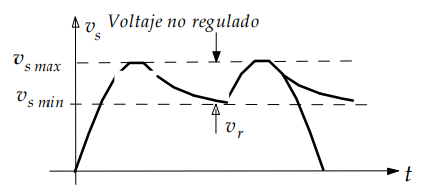
\includegraphics[width=0.75\linewidth]{src/Grafica.png}
    \caption{Relación del voltaje de entrada en el tiempo y voltaje de rizado.}
    \label{fig:fag4}
\end{figure}

Podemos definir entonces, que el voltaje de salida o reflejado en la carga es una función dependiente de variables como el voltaje de entrada, la corriente de la carga y la temperatura.



Fórmulas básicas necesarias para la manipulación del voltaje de rizo y control de capacitancia específica para un voltaje de salida específico en el regulador.

\noindent
\begin{minipage}[t]{0.48\textwidth}
\textbf{Fórmulas}
\begin{itemize}
    \item \textbf{Tensión de salida}
    \[
        v(t) = V_{\text{med}} + v_{\text{ripple}}(t)
    \]

    \item \textbf{Factor de rizado}
    \[
        F_R = \frac{V_{\text{ripple,rms}}}{V_{\text{med}}}
    \]


    \item \textbf{Relación $V_{\text{ripple,rms}}$ y $\Delta V$}
    \[
        V_{\text{ripple,rms}} = \frac{\Delta V}{2\sqrt{3}}
    \]

    \item \textbf{Factor de rizado con $\Delta V$}

    \[
        F_R = \frac{1}{V_{\text{med}}}\frac{I_L}{2\sqrt{3}fC}
    \]

    \item \textbf{Capacitancia requerida}
    \[
        C = \frac{I_L}{2\sqrt{3}fF_RV_{\text{med}}}
    \]
\end{itemize}
\end{minipage}%
\hfill
\begin{minipage}[t]{0.48\textwidth}
\textbf{Nomenclatura}
\begin{itemize}
    \item $V_{\text{med}}$: valor medio (DC) de la señal rectificada.
    \item $v_{\text{ripple}}(t)$: componente de rizado (promedio cero).
    \item $V_{\text{ripple,rms}}$: valor eficaz (rms) del rizado.
    \item $F_R$: factor de rizado.
    \item $V_p$: valor pico de la señal secundaria (antes de diodos).
    \item $\Delta V$: rizado pico a pico (peak-to-peak).
    \item $I_{\text{load}}$ o $I_L$: corriente de carga.
    \item $f_{\text{line}}$: frecuencia de la red (ej. 50 Hz).
    \item $f$: frecuencia de pulsos que recarga el condensador:
    \begin{itemize}
        \item media onda: $f = f_{\text{line}}$
        \item onda completa: $f = 2 f_{\text{line}}$
    \end{itemize}
    \item $C$: capacitancia del condensador de filtrado.
    \item $V_D$: caída en diodo(s) (corrección de $V_p$).
\end{itemize}
\end{minipage}



\section{Implementación}
\subsection{Fuente}


En esta sección se describe el diseño y cálculo de los componentes utilizados en la fuente de alimentación. Se emplean tres reguladores lineales \textbf{LM317}, dos configurados para entregar tensiones fijas de 3.3\,V y 5\,V, y uno ajustable entre 0--15\,V. 

El LM317 es un regulador de voltaje positivo ajustable cuya tensión de salida se define por:
\begin{equation}
    V_{out} = V_{ref}\left(1 + \frac{R_2}{R_1}\right) + I_{adj}R_2
\label{eq:lm317}
\end{equation}
donde:
$$V_{ref} \approx 1.25\,V \quad I_{adj} \approx 50\,\mu A $$

\subsection*{Resistencias}
Para calcular R2 en base a una R1 fija se utiliza la fórmula despejada de la ecuación \ref{eq:lm317}:
\begin{equation}
    R_2 = \dfrac{V_{out}-1.25}{1.25(\frac{1}{R_1}+I_{adj})}
\end{equation}
Aqui es donde se estuvo intentando con diferentes valores de resistencias para obtener los voltajes deseados. 
Hasta que llegamos a los siguientes valores:
\begin{itemize}
    \item Fuente de 5\,V: $R_1 = 330\magn{\Omega}, R_2 = 1k\magn{\Omega}$
    \item Fuente de 3.3\,V: $R_1 = 220\magn{\Omega}, R_2 = 360\magn{\Omega}$
    \item Fuente ajustable 0--15\,V: $R_1 = 470\magn{\Omega}, R_2 = 5K\magn{\Omega}$ (Potenciómetro)
\end{itemize}
De esta forma utilizaremos entonces resistencias comerciales con valores más cercanos y la resistencia de 360 $\Omega$ se obtiene por la serie de 330 $\Omega$ + 22 $\Omega$ + 10 $\Omega$. Quedando en 
\begin{itemize}
    \item \textbf{1R10}, \textbf{1R22} 
    \item \textbf{1R220}, \textbf{2R330} 
    \item \textbf{1R470}, \textbf{1R1K} 
    \item \textbf{1RV5K (Pot)}
\end{itemize}


\subsection*{Capacitores}
Para los valores de capacitancia de entrada se siguió la formula \ref{eq:cap}
\begin{equation}
    C=\dfrac{I_{CD}}{4f(V_{max}-V_{CD})}
    \label{eq:cap}
\end{equation}
Donde nosotros decidimos usar una corriente de 800 mA para el calculo de los capacitores como se puede observar en la siguiente expresión
$$
C=\dfrac{0.8}{4(120 Hz)(18 \sqrt{2} - V_{CD})}
$$
Donde $V_{CD}$ es el voltaje CD de cada regulador que se puede obtener por medio de la expresión \ref{eq:vcd}

\begin{equation}
    V_{CD} = V_{in} - V_{out} - V_{drop}
    \label{eq:vcd}
\end{equation}
Para el regulador LM317 se considera un $V_{drop}$ de 3.5\,V. Por lo tanto, los valores mínimos de $V_{CD}$ para cada regulador son:
\begin{itemize}
    \item Fuente de 5\,V: $C = 196.58 \mu \magn{F}$
    \item Fuente de 3.3\,V: $C = 178.67 \mu \magn{F}$
    \item Fuente ajustable 0--15\,V: $C = 479.123 \mu \magn{F}$
\end{itemize}
De forma que se seleccionaron capacitores electrolítico 220\,$\mu$F de 50 V \textbf{2CE220uF/50V} para ambas fuentes fijas y 680\,$\mu$F \textbf{1CE680uF/50V} para la fuente ajustable.

Para los capacitores de filtrado de entrada y salida se siguieron las recomendaciones del datasheet del LM317.
$$
C_{in}\text{: 0.1 uF} \quad C_{out}\text{: 1 uF}
$$
De esta forma se utilizarán 3 capacitores cerámicos \textbf{3CC0.1uF} y 3 electrolíticos \textbf{3CE1uF/50V} para cada regulador.


\subsection{Detector de Corto Circuito}
Para la detección del corto lo quisimos implementar mediante una resistencia shunt y un potenciometro. nosotros quisimos limitar la corriente hasta 800 mA, entonces el potenciometró detectará corto de 400-800 mA de acuerdo a la perilla. Esto permite una variedad de aplicaciones y personalización con respecto a la detección del corto.



Para poder lograr esto lo que nosotros diseñamos fue aplicar un divisor de voltaje de entre la resistencia de carga $R_L$ y la resistencia shunt con un valor de 0.15 $\magn{\Omega}$. Como se muestra en la figura \ref{fig:opan}, nosotros previamente limitamos la fuente hasta 800 mA la caida de tensión que habra en la resistencia shunt será de acuerdo a la ecuacion \ref{eq:om}. Con esta ecuación podemos definir el voltaje que dará con un rango de 60-120 mV como se puede observar en los casos de la ecuacion \ref{eq:casos} dandonos un rango de 0-10 mV. Resumiendo, esta salida nos da información con respecto a la corriente que esta circulando, información que es necesaria para detectar un corto.
\begin{equation}
    V= IR= I_L (0.1)
    \label{eq:om}
\end{equation}

\begin{equation}
\begin{aligned}        
    I&=0 \rightarrow V=0(0.1)=0  \magn{V}\\
    I&=800 mA \rightarrow V=800m\magn{A}(0.15)=120  m\magn{V}
\end{aligned}
\label{eq:casos}
\end{equation}


Ahora requeriremos de una señal de control que nos permita controlar la corriente máxima que varie entre 400-800 mA como habiamos dicho previamente. Para alimentar las señales de control utilizaremos un regulador de 5 V aislado de los voltajes que irán al usuario para esto usaremos el voltaje de 5 V proporcionado por nuestra fuente de control. Para obtener de 60-120 mV lo que haremos es utilizar un potenciometro de 10 K$\Omega$ para obtener valores de hasta 10 K$\Omega$, ahora para obtener el rango de 10-20 K $\Omega$ Simplemente añadiremos una resistencia de 10 K$\Omega$ en serie de esta forma permite desfasara el rango para obtener lo requerido. 


\begin{figure}[!h]
    \centering
    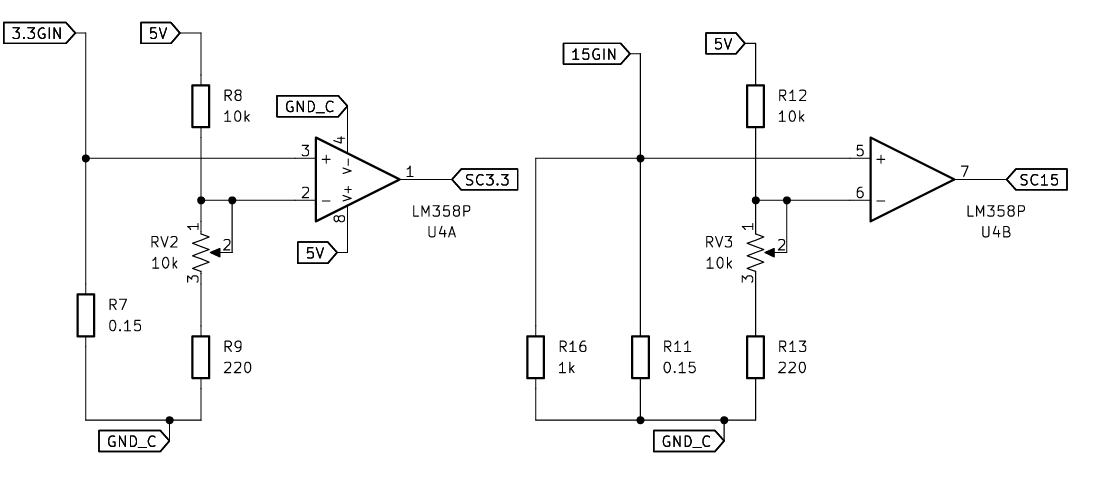
\includegraphics[width=1.0\linewidth]{src/opan.png}
    \caption{Configuración de detección de corto}
    \label{fig:opan}
\end{figure}

Para lograr obtener la señal de corto circuito utilizamos un comparador de voltaje, para ello utilizamos otro amplificador operacional \textbf{LM358P} configurado como comparador, en la entrada no inversora se conectará la señal proveniente de la resistencia shunt y en la entrada inversora se conectará la señal de control que definirá el umbral de corriente máxima. De esta forma cuando la tensión en la resistencia shunt supere el valor de referencia el comparador cambiará su salida a un nivel alto indicando un corto circuito. Este valor de referencia podra ser ajustado por medio de un potenciómetro que permitira variaciones entre 400-800 mA.

Se utilizarán dos detectores de corto circuito, uno para la salida ajustable y otro para las salida fija de 3.3. En caso de que alguno de los dos detectores detecte un corto circuito, la salida del latch cambiará a un nivel alto desactivando los reguladores y protegiendo la fuente y la carga conectada. Finalmente para lograr esto optamos por utilizar una compuerta or para unir las dos señales de corto circuito para esto lo logramos usando compuertas NANDS por medio de la siguiente ecuación \ref{eq:ornands}.
\begin{equation}
    \text{OR} (A,B) = \overline{\overline{A} \cdot \overline{B}}
    \label{eq:ornands}
\end{equation}




Para la implementación de la memoria, decidimos hacerla por medio de diseño digital y secuencial, para ello nosotros optamos por usar un Latch Set-Reset \textbf{CD4043B}, la lógica que decidimos implementar es que por medio de un botón pudiera retomar la operación normal de la fuente si y solo si dejo de haber corto, esto previene un mal funcionamiento y asegura la estabilidad de la fuente frente a sobrecargas y cortocircuito, para ello definimos las condicionales del latch.
$$
\begin{aligned}
S &\leftarrow \text{Corto Circuito}\\
&\boxed{S \leftarrow CC} \\
R &\leftarrow \text{Sin Corto Circuito y Boton Activo}\\
&\boxed{R \leftarrow !CC \& B}
\end{aligned}
$$
Nosotros decidimos implementar la logica por medio de NANDS creadas por ANDs y NOT debido a disponibilidad de componentes y optimización de espacio. La ecuación final del Reset se implementa entonces por los integrados \textbf{74LS08} de 4 ANDS y \textbf{74LS04} de 6 NOTS como se puede apreciar en la figura \ref{fig:Combi}
\begin{lstlisting}
    T1 <= !(CC & CC);
    T2 <= !(T1 & SW);
    R  <= !(T2 & T2);
\end{lstlisting}

\begin{figure}[!h]
    \centering
    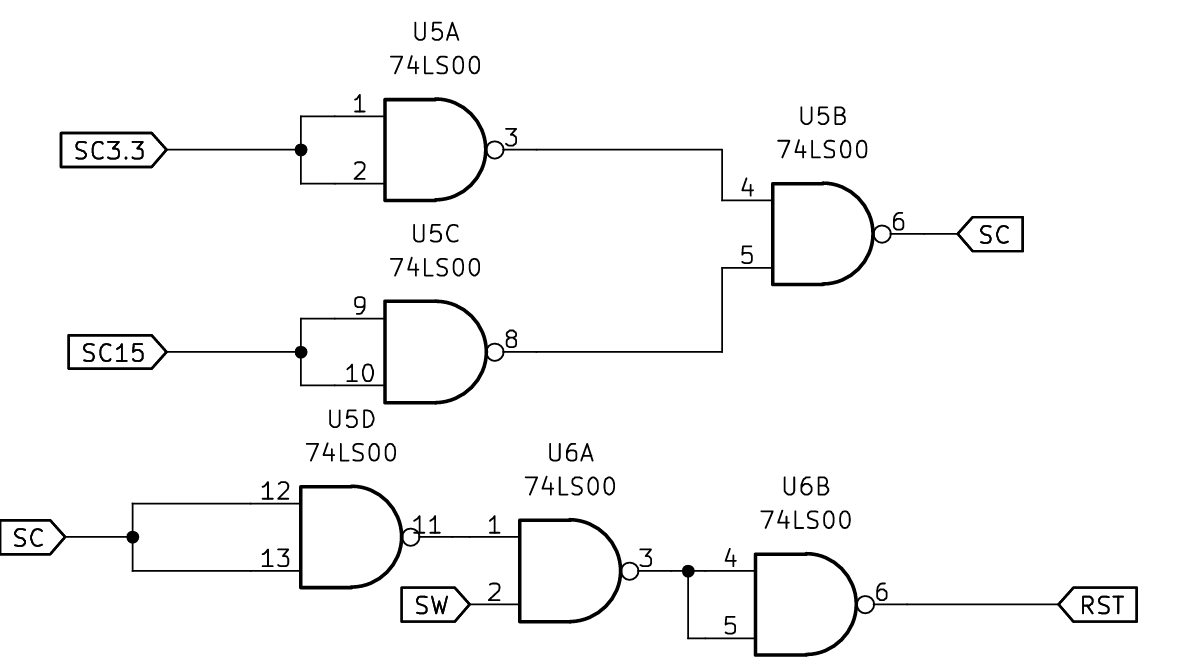
\includegraphics[width=.80\linewidth]{src/Combi.png}
    \caption{Lógica Combinacional}
    \label{fig:Combi}
\end{figure}


Finalmente, la salida del latch se conectará a un transistor NPN \textbf{2N2222} configurado como interruptor para controlar la activación de los reguladores por medio de un relevador con señal de 5V. Cuando la salida del latch esté en nivel bajo, el transistor conducirá y permitirá el paso de corriente a los reguladores, habilitándolos. En caso contrario, el transistor estará en corte, desactivando los reguladores y protegiendo la fuente.
Para el calculo de la resistencia de base consideramos la ganancia del transistor $h_{FE} = 360$ y una corriente de colector máxima de 120 mA para el relevador. Por lo tanto, la corriente de base necesaria será 
$$I_B = \dfrac{I_C}{h_{FE}} = \dfrac{120 mA}{360} \approx 0.3 mA$$
Utilizando una tensión de base de 5 V y una caída de tensión $V_{BE}$ de 0.7 V, la resistencia de base se calcula como:
\begin{equation*}
    R_B = \dfrac{V_{in} - V_{BE}}{I_B} = \dfrac{5 V - 0.7 V}{0.3 mA} \approx 12.9k \Omega
\end{equation*}
Se seleccionará una resistencia comercial de 15 k$\Omega$ \textbf{1R15K} para limitar la corriente de base del transistor. Por seguridad se calculó cuanto incrementaria la corriente con el nuevo valor de resistencia.
$$
I_B = \dfrac{5 V - 0.7 V}{15 k\Omega} \approx 0.29 mA
$$
Siendo una corriente adecuada para activar el transistor sin exceder sus límites.

Esto daría como resultado un circuito como lo muestra la figura \ref{fig:Control} para la entrada de Reset, nos gustaria hacer mención sobre como antes de decidirnos por la alternativa de un latch exploramos otras alternativas como lo fue utilizar un SCR o inclusive con un comportamiento secuencial disparado por un reloj, pero debido a optimización del espacio decidimos implementarlo de la forma con latch.

\begin{figure}[!h]
    \centering
    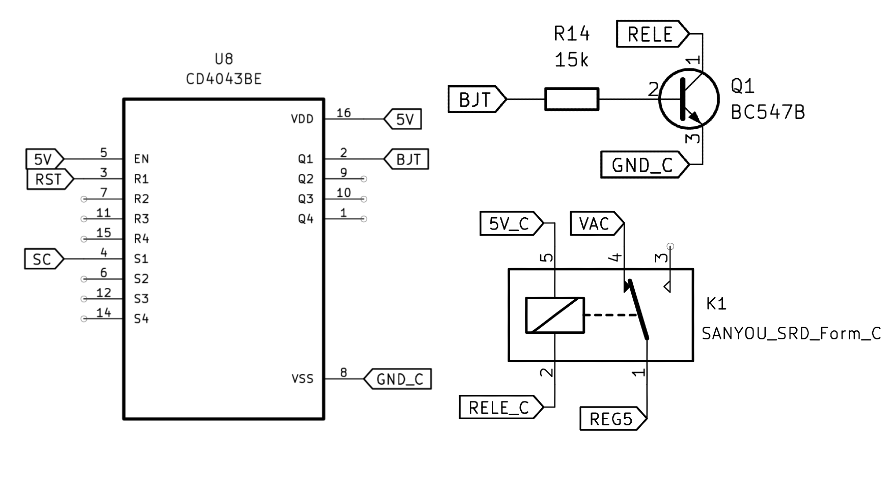
\includegraphics[width=1.0\linewidth]{src/Control.png}
    \caption{Circuito Control-Potencia}
    \label{fig:Control}
\end{figure}
\section{Análisis de Costos y Especificaciones}

Para la construcción de la fuente de voltaje lineal con protección contra cortocircuito se adquirieron los componentes mostrados en la Tabla \ref{tab:bom}. Se consideran los elementos electrónicos utilizados para la regulación, rectificación, sensado de corriente, protección y etapa de control. Los precios fueron estimados con base en proveedores locales y tiendas de componentes electrónicos con valores promedio comerciales.

    
\begin{table}[htbp]
\caption{Lista de materiales y costos del proyecto}
\label{tab:bom}
\centering
\begin{tabular}{clrr}
\hline
\textbf{Cant.} & \textbf{Descripción/Modelo} & \textbf{P. Unit. (MXN)} & \textbf{Subtotal (MXN)} \\
\hline
1 & Transformador 18V/2A & \$300.00 & \$300.00 \\
1 & Carcasa 15$\times$25 cm & \$128.45 & \$128.45 \\
1 & Voltímetro & \$78.00 & \$78.00 \\
3 & Disipadores de Calor & \$16.00 & \$48.00 \\
3 & Regulador LM317T & \$16.00 & \$48.00 \\
9 & Borneras 2$\times$1 & \$5.25 & \$47.25 \\
2 & Potenciómetro k$\Omega$ & \$22.50 & \$45.00 \\
2 & TTL NAND 74LS00 & \$22.50 & \$45.00 \\
1 & Relé 5V-127 & \$32.50 & \$32.50 \\
2 & Placa Fenólica & \$14.00 & \$28.00 \\
4 & Jack Banana & \$6.00 & \$24.00 \\
1 & Resistencias 0.15 $\Omega$ & \$20.00 & \$20.00 \\
1 & CMOS latch CD4043BE & \$17.50 & \$17.50 \\
2 & Electrolítico 220 $\mu$F & \$7.75 & \$15.50 \\
1 & Puente rectificador KBP206G & \$14.75 & \$14.75 \\
1 & Porta Fusible Europeo & \$12.93 & \$12.93 \\
1 & Potenciómetro 5 k$\Omega$ & \$12.00 & \$12.00 \\
1 & Electrolítico 680 $\mu$F & \$7.75 & \$7.75 \\
3 & Electrolítico 1 $\mu$F & \$2.50 & \$7.50 \\
1 & Plug Banana & \$5.60 & \$5.60 \\
1 & Op. Amp LM358P & \$5.50 & \$5.50 \\
3 & Cerámico 0.1 $\mu$F & \$1.75 & \$5.25 \\
4 & Resistencias 220 $\Omega$ & \$1.25 & \$5.00 \\
1 & Fusible 250 mA & \$4.00 & \$4.00 \\
1 & Transistor BC547B & \$3.50 & \$3.50 \\
2 & Resistencias 1 k$\Omega$ & \$1.25 & \$2.50 \\
2 & Resistencias 10 k$\Omega$ & \$1.25 & \$2.50 \\
2 & Resistencias 330 $\Omega$ & \$1.25 & \$2.50 \\
1 & Resistencias 10 $\Omega$ & \$1.25 & \$1.25 \\
1 & Resistencias 15 k$\Omega$ & \$1.25 & \$1.25 \\
1 & Resistencias 22 $\Omega$ & \$1.25 & \$1.25 \\
1 & Resistencias 470 $\Omega$ & \$1.25 & \$1.25 \\
\hline
\multicolumn{3}{r}{\textbf{Total:}} & \textbf{\$1,067.48} \\
\hline
\end{tabular}
\end{table}

\noindent\textbf{Características del prototipo:}
\begin{itemize}
    \item \textbf{Tipo de fuente:} Lineal regulada con protección por cortocircuito.
    \item \textbf{Entradas:} 127VAC a 60Hz.
    \item \textbf{Voltaje secundario del transformador:} 18Vac.
    \item \textbf{Salidas disponibles:}
    \begin{itemize}
        \item 3.3V DC fija (LM317 configurado).
        \item 5V DC fija (LM317 configurado).
        \item 0–15V DC ajustable mediante potenciómetro.
    \end{itemize}
    \item \textbf{Corriente máxima de operación:} 800mA (limitada por shunt y comparador).
    \item \textbf{Protección contra cortocircuito:} Comparador LM358 + Latch CD4043B + etapa de control con relevador.
    \item \textbf{Modo de recuperación:} Manual mediante pulsador (Reset), sólo si no existe corto.
    \item \textbf{Ripple esperado después de filtrado:} $<$5\% para cargas dentro del rango.
    \item \textbf{Aplicaciones:} Laboratorio, pruebas electrónicas, prototipos educativos.
\end{itemize}
El costo total estimado del proyecto fue de aproximadamente \textbf{{\$} 1070 MXN}, lo cual lo convierte en un diseño accesible para aplicaciones educativas y de laboratorio. El uso de reguladores lineales y protección discreta permitió reducir costos sin comprometer la funcionalidad principal del sistema.

\vspace{0.4cm}

\subsection*{Especificaciones Técnicas del Prototipo}


Con estas características, la fuente fabricada cumple con los objetivos de regulación estable, operación segura ante sobrecargas y capacidad multi-voltaje para alimentar circuitos digitales y analógicos en prácticas académicas.


\section{Fallas Típicas}

Durante el desarrollo e implementación de la fuente con protección contra cortocircuito se identificaron diversas fallas recurrentes asociadas tanto al diseño como al montaje del circuito. A continuación se describen las principales fallas típicas encontradas y su causa raíz:

\subsection*{1. Activación falsa del detector de cortocircuito}
En algunos casos el sistema detectó cortocircuito aun cuando la carga era adecuada. Esto se debe principalmente a:
\begin{itemize}
    \item Ruido eléctrico en la línea de sensado.
    \item Valores muy pequeños de voltaje en la resistencia shunt.
    \item Falta de desacoplos adecuados en la etapa de amplificación.
\end{itemize}
Para evitar este problema es recomendable filtrar la señal mediante un capacitor de desacoplamiento o aumentar ligeramente la ganancia del amplificador operacional.

\subsection*{2. Protección que no se activa correctamente}
Este problema ocurre cuando el valor del potenciómetro o el umbral de corte del amplificador no coincide con el rango esperado de corriente. Las causas principales son:
\begin{itemize}
    \item Ajuste incorrecto del potenciómetro de referencia.
    \item Saturación del amplificador operacional.
    \item Selección de componentes con tolerancias altas.
\end{itemize}


\subsection*{3. Inestabilidad en la etapa de memoria (Latch)}
En algunos casos la memoria no retiene correctamente el estado de protección. Esto se debe generalmente a:
\begin{itemize}
    \item Señales de entrada con rebotes.
    
    \item Mala distribución de tierra o interferencia en la señal.
\end{itemize}


En resumen, la mayoría de las fallas estuvieron relacionadas con ruido, tolerancias de los componentes y el diseño del trazado en PCB. Considerar reglas de ruteo, diseño de tierra adecuado y desacoplos cercanos permite minimizar estos problemas y garantizar una operación más robusta del sistema.


%----------------------------------------------------------------------
\section{Cumplimiento Normativo: NOM-001-SCFI-2018 para Fuentes de Alimentación Externa}
\label{sec:normatividad}

La fuente de alimentación desarrollada cumple con los requisitos establecidos en el Apéndice I de la NOM-001-SCFI-2018, específicos para Fuentes de Alimentación Externa (FAE). A continuación se detalla cómo el diseño satisface cada uno de los requisitos aplicables.

\subsection{Marcado e Instrucciones (I.3)}

El equipo cumple con los requisitos de marcado conforme a la normativa:
\begin{itemize}
    \item Todos los textos de seguridad están redactados en español, cumpliendo con el requisito obligatorio.
    \item Las unidades de medida empleadas (V, A, $\Omega$, F) cumplen con la NOM-008-SCFI-2002.
    \item El marcado general del producto incluye especificaciones técnicas bilingües (español/inglés) donde es aplicable.
\end{itemize}

\subsection{Interfaz de Potencia (I.2)}

La conexión eléctrica del equipo cumple con los incisos 1.6.2, 1.6.3 y 1.6.4 de la NMX-I-60950-1-NYCE-2015:
\begin{itemize}
    \item Conexiones de entrada y salida claramente identificadas.
    \item Terminales de conexión con capacidad adecuada para la corriente nominal.
    \item Aislamiento apropiado entre circuitos primarios y secundarios mediante el transformador.
\end{itemize}

\subsection{Protección contra Choques Eléctricos (I.4)}

El diseño garantiza la protección del usuario conforme a los incisos 2.1 y 2.2 de la norma de referencia:
\begin{itemize}
    \item Las partes conductoras accesibles (conectores banana, borneras) operan a tensiones de seguridad extra baja (SELV).
    \item El gabinete aísla completamente las partes vivas peligrosas del usuario.
    \item No existen partes conductoras desnudas accesibles en condiciones normales de operación.
\end{itemize}

\subsection{Circuitos para Limitar Corriente (I.5)}

La fuente incorpora múltiples mecanismos de protección:
\begin{itemize}
    \item \textbf{Fusible de entrada} (250 mA): Protege contra sobrecorrientes en el primario.
    \item \textbf{Regulador LM317T}: Incluye protección térmica y limitación de corriente integrada.
    \item \textbf{Resistencia de sensado} (0.15 $\Omega$): Permite monitoreo y limitación de corriente de salida.
    \item Los valores límite no se exceden bajo condiciones normales ni de falla.
\end{itemize}


\subsection{Requisitos Térmicos (I.13)}

El manejo térmico del equipo garantiza operación segura:
\begin{itemize}
    \item \textbf{Disipadores de calor}: Instalados en los reguladores LM317T para mantener temperaturas seguras al tacto.
    \item Las superficies externas accesibles no superan los límites de temperatura establecidos.
    \item Los componentes y aislamientos están seleccionados para no degradarse durante la vida útil del equipo.
\end{itemize}


\subsection{Resumen de Cumplimiento}

La Tabla~\ref{tab:cumplimiento} presenta un resumen del cumplimiento normativo de la fuente de alimentación.

\begin{table}[htbp]
\caption{Resumen de cumplimiento con NOM-001-SCFI-2018, Apéndice I (FAE)}
\label{tab:cumplimiento}
\centering
\begin{tabular}{lcc}
\hline
\textbf{Requisito} & \textbf{Inciso} & \textbf{Cumple} \\
\hline
Marcado e Instrucciones & I.3 & \checkmark \\
Interfaz de Potencia & I.2 & \checkmark \\
Protección contra Choques Eléctricos & I.4 & \checkmark \\
Circuitos para Limitar Corriente & I.5 & \checkmark \\
Requisitos Térmicos & I.13 & \checkmark \\
\hline
\end{tabular}
\end{table}



\section{Conclusiones}

El presente proyecto permitió diseñar e implementar una fuente de alimentación lineal con salidas de 3.3V, 5V y 0--15V ajustable, incluyendo un sistema de protección contra cortocircuito funcional. A partir del desarrollo realizado, se pueden establecer las siguientes conclusiones:

\begin{enumerate}
    \item \textbf{Diseño del regulador:} La implementación de reguladores LM317 demostró ser una solución efectiva para obtener voltajes estables y configurables. Los cálculos de resistencias permitieron alcanzar los valores de salida requeridos con precisión aceptable para aplicaciones de laboratorio.
    
    \item \textbf{Sistema de protección:} El circuito de detección de cortocircuito basado en resistencia shunt y comparador LM358 cumple su función de manera confiable. La combinación con el latch CD4043B garantiza que la protección se mantenga activa hasta que el usuario intervenga conscientemente, previniendo daños tanto a la fuente como a la carga.
    
    \item \textbf{Cumplimiento normativo:} La fuente diseñada satisface al menos dos especificaciones de la NOM-001-SCFI-2018 para fuentes de alimentación externa, específicamente en los requisitos de protección contra choques eléctricos (I.4) y circuitos para limitar corriente (I.5), lo cual valida su seguridad para uso en entornos controlados.
    
    \item \textbf{Análisis económico:} Con un costo total aproximado de \$1,070 MXN, el dispositivo representa una alternativa accesible comparada con fuentes comerciales de características similares, las cuales suelen superar los \$2,000 MXN en el mercado.
    
    \item \textbf{Aprendizaje técnico:} El proyecto integró conocimientos de electrónica analógica (reguladores, amplificadores operacionales), electrónica digital (lógica combinacional, latches) y diseño de potencia (manejo térmico, protecciones), demostrando la importancia de un enfoque multidisciplinario en el diseño de sistemas electrónicos.
    
    \item \textbf{Áreas de mejora:} Para futuras iteraciones se recomienda implementar indicadores visuales del estado de cada salida, mejorar el filtrado de ruido en la etapa de sensado, y considerar el uso de reguladores conmutados para mejorar la eficiencia energética.
\end{enumerate}

En conclusión, el proyecto cumplió satisfactoriamente con los objetivos planteados, generando un prototipo funcional que demuestra la aplicación práctica de los conceptos estudiados en la materia de Dispositivos Electrónicos.

\section{Retroalimentación personal}
\begin{itemize}
    \item \textbf{Das:}
    
    Esta materia en lo particular me pareció un tanto complicada al inicio porque tenía que analizar los circuitos con una lógica diferente a la física y a las matemáticas, representó un gran desafío para mi pero se me hizo interesante y considero que con el diseño del proyecto se demostró los conocimientos al permitirnos diseñar toda una fuente desde la parte de los reguladores y también unir ciertos conceptos como lo fue la lógica combinacional. 
    \item \textbf{Iker Navarrete:}
    
     Me gustaria que diera muchos mas ejercicios como tareas esporadicas y con retroalimentacion en clase, me gustaron los temas vistos y que el profesor dominaba el tema de la materia, el proyecto siento que pudimos haber visto mas la parte teorica o al menos senti que debio de haber un poco mas de acompañamiento en el ultimo parcial, más que nada para aplicarlo mucho para la fuente sentí que estuvo muy justo de tiempo 

    
    \item \textbf{Iker García:}
    
    Esta materia realmente la disfrute ya que fueron ideas y componentes completamente nuevos usando metodos ya conocidos, para mi la dificultad de esta materia es el hecho que para entenderle de una gran manera se requiere el hacer muchos ejercicios y con variaciones ya que con un poco que cambie el circuito cambian los calculos y pues mas que nada tener el tiempo para darle esa dedicacion y con la carga de otras materias realmente se me hace pesado. Siento que el tema de recortadores, sujetadores y diodos en general se puede visualisar mejor con mas simulaciones y animaciones ya que en hojas es menos visual.
    \item \textbf{Kevin:}
    
    Esta chida, aprendi mucho sobre electronica basica manejo de diodos, transistores y un poco de diseño de circuitos, a mi punto de vista la materia me pareció legal la verdad creí que estaría mas díficil, el proyecto fue laborioso pero adecuado. Considero que la materia se pudo haber llevado en semestres anteriores.
\end{itemize}

\begin{thebibliography}{4}

\bibitem{huircan2012}
Huirc\'{a}n, J. (2012). \textit{Reguladores de voltaje}. Recuperado de: http://quidel.inele.ufro.cl/jhuircan/PDF\_CTOSII/reguieee.pdf

\bibitem{miyara2002}
Miyara, F. (2002). \textit{Rectificaci\'{o}n}. Argentina: Riobamba, p. 245.

\bibitem{transformadores}
P\'{e}rez-Londo\~{n}o, S. M. (2022). \textit{Transformadores el\'{e}ctricos}. Google Books. Recuperado de: https://books.google.com.mx/books?id=42SXEQAAQBAJ

\bibitem{rendon_rectificadores}
Rend\'{o}n, J. F. G. (s.f.). \textit{Rectificadores y Filtros}. Universidad de Antioquia.

\end{thebibliography}

\end{document}
